% ============================================================================
% Problem Formulation
% ============================================================================

\subsection{Notation and Measurement Model}

We define a global \emph{world frame} $\mathcal{W}$ (ENU convention,
$Z$-axis anti-parallel to gravity) and a \emph{body frame} $\mathcal{B}$
fixed to the rover.
$N$ anchors at known positions $\mathbf{a}_i \in \mathbb{R}^d$
($i = 1,\ldots,N$, $d \in \{2,3\}$) range to a mobile tag at
position $\mathbf{p}(t) \in \mathbb{R}^d$.

Each DS-TWR exchange produces a scalar range measurement
\begin{equation}
  \rho_i = \|\mathbf{p} - \mathbf{a}_i\|_2 + \delta_i + \varepsilon_i,
  \label{eq:range_model}
\end{equation}
where $\delta_i$ captures systematic bias (antenna delay, NLOS path
lengthening) and $\varepsilon_i \sim \mathcal{N}(0,\sigma_i^2)$ with
$\sigma_i \approx 0.05$--$0.15$\,m under LOS.
The goal is the weighted maximum-likelihood position:
\begin{equation}
  \hat{\mathbf{p}} = \arg\min_{\mathbf{p}} \sum_{i=1}^{N}
    w_i \bigl(\|\mathbf{p} - \mathbf{a}_i\|_2 - \rho_i\bigr)^2,
  \label{eq:multilateration}
\end{equation}
where $w_i \leq 1$ downweight NLOS-contaminated anchors (\S\ref{sec:nlos}).

\subsection{Trilateration: 2D and 3D Geometry}

\begin{figure}[t]
  \centering
  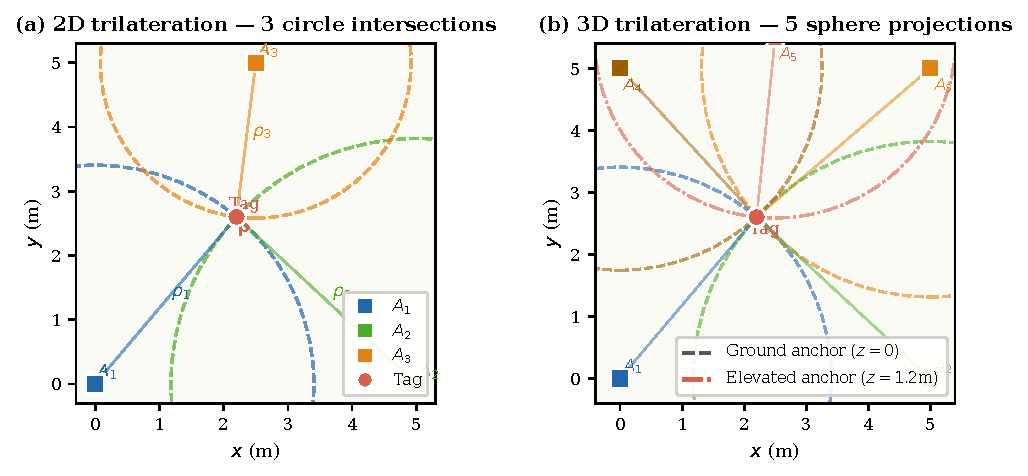
\includegraphics[width=\columnwidth]{figures/trilateration_geometry.pdf}
  \caption{Trilateration geometry.
  \textit{(a)}~2D: each anchor constrains the tag to a circle; the position is
  the common intersection.
  \textit{(b)}~3D top view: five anchors determine the tag in 3D; elevated
  anchor $A_5$ breaks planar degeneracy and makes height $p_z$ observable.}
  \label{fig:trilat_geometry}
\end{figure}

\textbf{2D case.}
Each range $\rho_i$ places the tag on a circle centred at $\mathbf{a}_i$
(Fig.~\ref{fig:trilat_geometry}a):
\begin{equation}
  (p_x - a_{i,x})^2 + (p_y - a_{i,y})^2 = \rho_i^2.
  \label{eq:circles}
\end{equation}
Three or more non-collinear anchors give a unique intersection.

\textbf{3D case.}
Each range defines a sphere (Fig.~\ref{fig:trilat_geometry}b):
\begin{equation}
  (p_x - a_{i,x})^2 + (p_y - a_{i,y})^2 + (p_z - a_{i,z})^2 = \rho_i^2.
  \label{eq:spheres}
\end{equation}
Four non-coplanar anchors give a unique intersection.
In our deployment, anchor $A_5$ is elevated ($z = 1.2$\,m) while
$A_1$--$A_4$ are near the floor, breaking planar degeneracy and making
$p_z$ observable from trilateration alone.
Observability requires $N \geq 3$ non-collinear anchors for $d=2$
and $N \geq 4$ non-coplanar anchors for $d=3$.

\subsection{Iterative Solver and Output Covariance}
\label{sec:lm_derivation}

Subtracting the first anchor's equation from each subsequent one
eliminates the quadratic $\|\mathbf{p}\|^2$ term, yielding a linear
system $\mathbf{A}\hat{\mathbf{p}}_0 = \mathbf{b}$:
\begin{align}
  A_{i-1,\cdot} &= 2\bigl(a_{i,x}-a_{1,x},\ a_{i,y}-a_{1,y}
    [,\ a_{i,z}-a_{1,z}]\bigr), \label{eq:lin_A}\\
  b_{i-1} &= \rho_1^2 - \rho_i^2 + \|\mathbf{a}_i\|^2
    - \|\mathbf{a}_1\|^2, \label{eq:lin_b}
\end{align}
giving the closed-form warm-start
$\hat{\mathbf{p}}_0 = (\mathbf{A}^\top\mathbf{A})^{-1}\mathbf{A}^\top\mathbf{b}$.
Starting from $\hat{\mathbf{p}}_0$, Levenberg--Marquardt refines the
solution iteratively.
The residual $f_i = \|\mathbf{p}-\mathbf{a}_i\|_2 - \rho_i$ has
Jacobian rows
\begin{equation}
  J_{i,k} = \frac{p_k - a_{i,k}}{\|\mathbf{p}-\mathbf{a}_i\|_2},
  \label{eq:jacobian}
\end{equation}
the unit direction from anchor $i$ to the tag.
Each iteration solves the damped weighted normal equation
\begin{equation}
  \bigl(\mathbf{J}^\top\mathbf{W}\mathbf{J} + \lambda\mathbf{D}\bigr)
  \Delta\mathbf{p} = -\mathbf{J}^\top\mathbf{W}\mathbf{f},
  \label{eq:lm_step}
\end{equation}
until $\|\Delta\mathbf{p}\|_2 < 10^{-5}$\,m or 50 iterations are reached.
The output covariance fed to the EKF is
\begin{equation}
  \hat{\boldsymbol{\Sigma}} = \hat{\sigma}^2
    (\mathbf{J}^\top\mathbf{W}\mathbf{J})^{-1}, \quad
  \hat{\sigma}^2 = \frac{\mathbf{f}^\top\mathbf{W}\mathbf{f}}{N-d},
  \label{eq:lm_cov}
\end{equation}
so a high-residual or heavily down-weighted fix automatically inflates
the EKF measurement noise, reducing its influence on the state estimate.
